\appendixtitleon

\chapter{Artery}

\section{code verification}
\label{app:VV-artery}


In this work, code verification is performed by considering a cube $B = [0,1]^3$ and a manufactured displacement field taken as 
\begin{equation}
    \bfu^{\textnormal{MMS}}(\bfx) = (-0.01\exp(x_3), 0, 0)^T\,.
\end{equation}
Dirichlet boundary conditions in accordance with the above solution are prescribed on all boundaries. A body force is defined such that the manufactured solution corresponds to the nonlinear boundary value problem defined in Section \ref{subsec:def-NBVP}. The convergence order is measured by the $L^2$-norm of the difference between the approximation and the manufactured solution. The $h$-convergence of the norm is shown in Fig.~\ref{fig:mms}, and a third-order convergence rate is observed as expected.
\begin{figure}[ht!]
    \begin{center}
        \includegraphics[trim = {2cm 9cm 2cm 9cm}, clip, width = 0.6\textwidth]{MMS-Convergence.pdf}
    \end{center}
    \caption[Convergence of the $L^2$ error for the manufactured solution.]{Convergence of the $L^2$ error ($h$-refinement) for the manufactured solution.}
    \label{fig:mms}
\end{figure}

\section{Strategy for Solving the Fractional Stochastic Partial Differential Equation}\label{sec:solver-SPDE}
For the sake of self-consistency, the numerical strategy to solve the anisotropic fractional stochastic partial differential equation
\begin{equation}
    (\gamma^2 \mathcal{I} -\langle \nabla, \bs{D}\nabla\rangle)^{\alpha/2} U = \dot{W}\,,
    \label{eq:spdeH-app}
\end{equation}
is recalled in this appendix. Following \cite{Lindgren2011}, a finite-dimensional representation associated with a set $\{\psi_i\}_{i=1}^{N}$ of piecewise linear basis functions (with a mesh comprising $N$ nodes) is introduced as follows:
\begin{equation}
U(\bs{x}) = \sum_{i=1}^{N} U_i \psi_i(\bs{x})\,.
\end{equation}
Let $\bs{U} = (U_1, \ldots, U_N)^T$ be the Gaussian random vector of nodal values. For $\alpha = 2$, it was shown in the above reference that the weak Galerkin stochastic solution satisfies
\begin{equation}
    \bs{U} \sim \mathcal{N}(\bs{0}_N, \bs{\Sigma})\,,
\end{equation}
where the covariance matrix $\bs{\Sigma}$ is given by 
\begin{equation}
    \bs{\Sigma} = \left(\kappa^2 \bs{M} + \bs{G}\right)^{-1} \bs{M} \left(\kappa^2 \bs{M} + \bs{G}\right)^{-1}]\,,
\end{equation} 
with
\begin{equation}
M_{ij} = \int_{\Omega} \psi_i(\bs{x})\psi_j(\bs{x})\,d\bs{x}
\label{eq:M}
\end{equation}
and
\begin{equation}
G_{ij} = \int_{\Omega} \langle \bs{\nabla}\psi_i(\bs{x}), \bs{D}(\bs{x})\bs{\nabla}\psi_j(\bs{x})\rangle \, d\bs{x}
\end{equation}
for $1 \leqslant i,j \leqslant N$, respectively. For computational efficiency, the sampling task is then usually recast using the precision matrix 
\begin{equation}
    \bs{\Sigma}^{-1} = \left(\kappa^2 \bs{M} + \bs{G}\right) \bs{M}^{-1} \left(\kappa^2 \bs{M} + \bs{G}\right)\,,
\end{equation}
where $\bs{M}^{-1}$ can be evaluated by applying a lumping procedure. For $\alpha \neq 2$, recursive formula can be applied, see \cite{Lindgren2011}.


\section{Reduced-Order Model Solutions}
In this Appendix, additional solution snapshots are provided, together with absolute errors, to assess the accuracy of the presented frameworks.
\begin{figure}[!htb]
     \begin{center}
        \begin{subfigure}[b]{0.23\textwidth}
            \begin{center}
                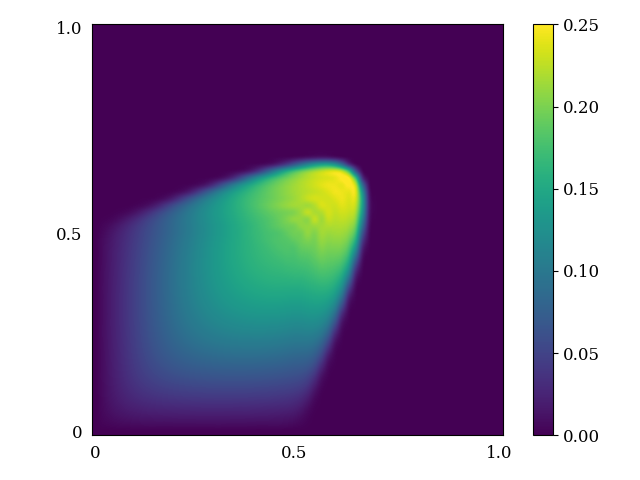
\includegraphics[trim = {0, 0, 3cm, 0}, clip, width=\textwidth]{X-rom-LE-DAE-5.png}
            \end{center}
            \caption{Solution $r = 5$}
        \end{subfigure}
   \begin{subfigure}[b]{0.23\textwidth}
            \begin{center}
                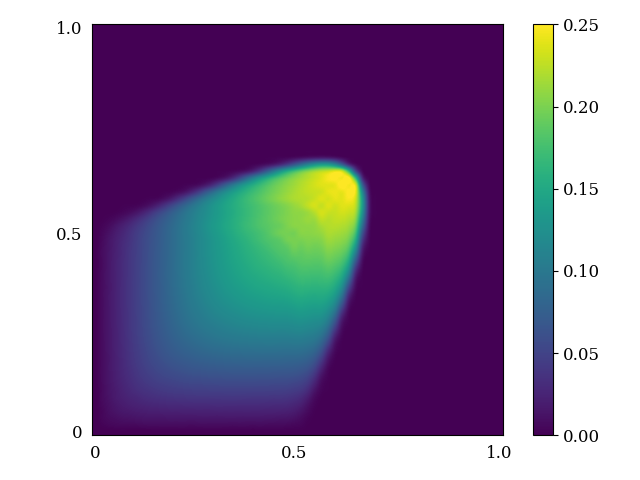
\includegraphics[trim = {0, 0, 3cm, 0}, clip, width=\textwidth]{X-rom-LE-DAE-10.png}
            \end{center}
            \caption{Solution $r = 10$}
        \end{subfigure}
   \begin{subfigure}[b]{0.23\textwidth}
            \begin{center}
                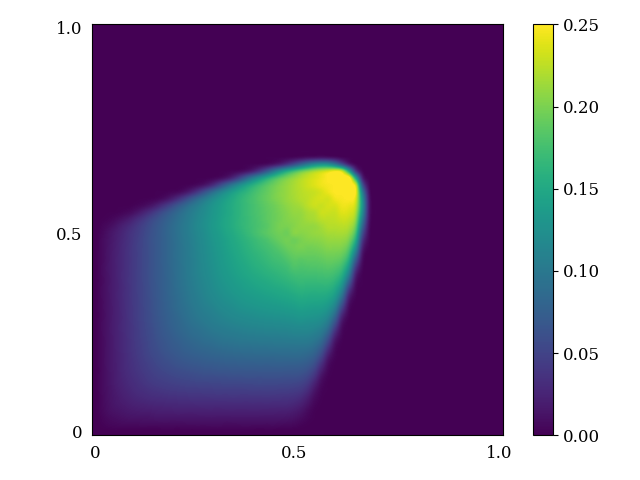
\includegraphics[trim = {0, 0, 3cm, 0}, clip, width=\textwidth]{X-rom-LE-DAE-15.png}
            \end{center}
            \caption{Solution $r = 15$}
        \end{subfigure}
   \begin{subfigure}[b]{0.23\textwidth}
            \begin{center}
                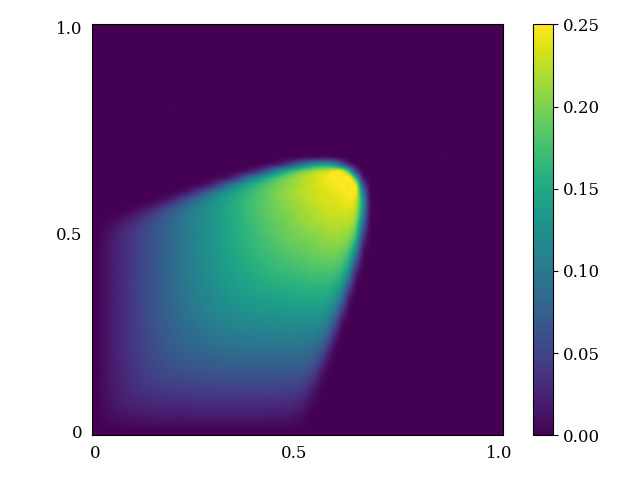
\includegraphics[trim = {0, 0, 3cm, 0}, clip, width=\textwidth]{X-rom-LE-DAE-20.png}
            \end{center}
            \caption{Solution $r = 20$}
        \end{subfigure}\\  
        \begin{subfigure}[b]{0.23\textwidth}
            \begin{center}
                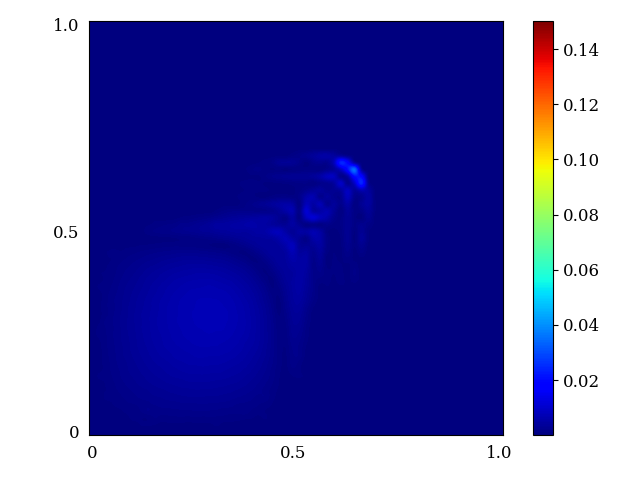
\includegraphics[trim = {0, 0, 3cm, 0}, clip, width=\textwidth]{X-rom-LE-DAE-5-abs-err.png}
            \end{center}
            \caption{Absolute error $r = 5$}
        \end{subfigure}  
        \begin{subfigure}[b]{0.23\textwidth}
            \begin{center}
                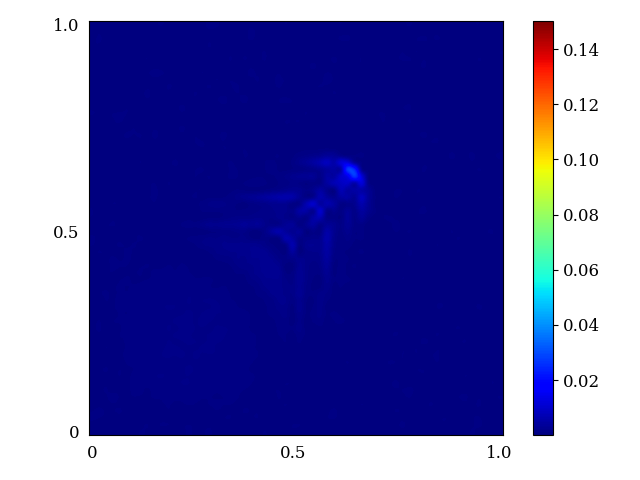
\includegraphics[trim = {0, 0, 3cm, 0}, clip, width=\textwidth]{X-rom-LE-DAE-10-abs-err.png}
            \end{center}
            \caption{Absolute error $r = 10$}
        \end{subfigure}   
        \begin{subfigure}[b]{0.23\textwidth}
            \begin{center}
                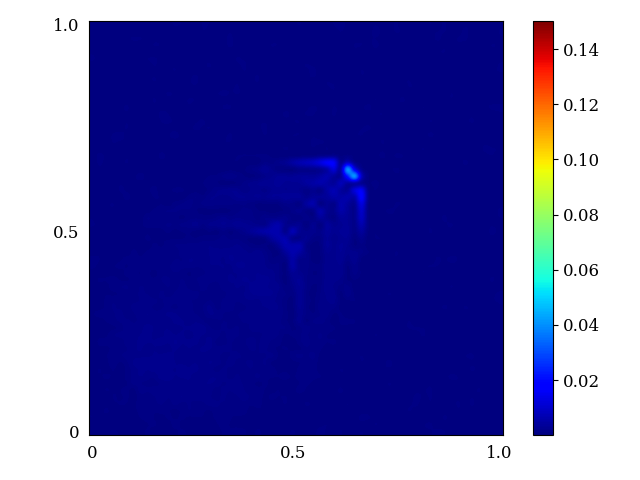
\includegraphics[trim = {0, 0, 3cm, 0}, clip, width=\textwidth]{X-rom-LE-DAE-15-abs-err.png}
            \end{center}
            \caption{Absolute error $r = 15$}
        \end{subfigure}    
        \begin{subfigure}[b]{0.23\textwidth}
            \begin{center}
                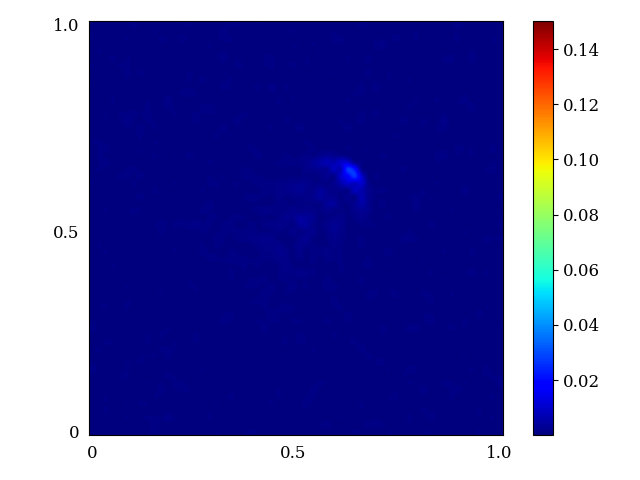
\includegraphics[trim = {0, 0, 3cm, 0}, clip, width=\textwidth]{X-rom-LE-DAE-20-abs-err.png}
            \end{center}
            \caption{Absolute error $r = 20$}
        \end{subfigure}
     \end{center}
     \caption[Solutions and pointwise errors for LE-DAE-DNNOp.]{Solutions (a, b, c, d) and pointwise errors (e, f, g, h) for LE-DAE-DNNOp with different latent space dimensions.}
        \label{fig: ledae-burger}
\end{figure}

\begin{figure}[!htb]
     \begin{center}
        \begin{subfigure}[b]{0.23\textwidth}
            \begin{center}
                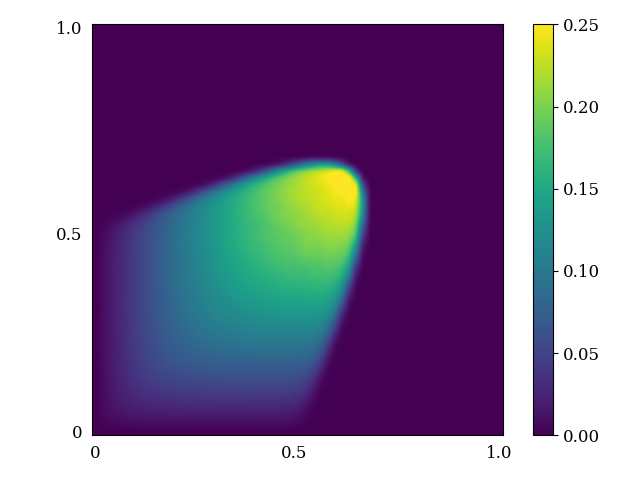
\includegraphics[trim = {0, 0, 3cm, 0}, clip, width=\textwidth]{X-rom-LE-SAE-5.png}
            \end{center}
            \caption{Solution $r = 5$}
        \end{subfigure}
   \begin{subfigure}[b]{0.23\textwidth}
        \begin{center}
            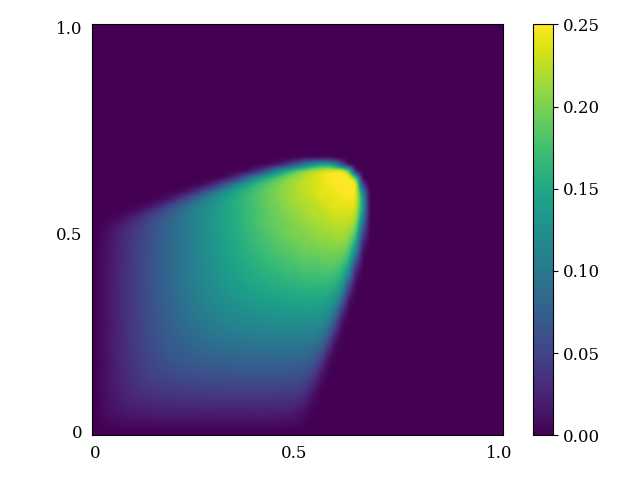
\includegraphics[trim = {0, 0, 3cm, 0}, clip, width=\textwidth]{X-rom-LE-SAE-10.png}
        \end{center}
            \caption{Solution $r = 10$}
        \end{subfigure}
   \begin{subfigure}[b]{0.23\textwidth}
       \begin{center}
        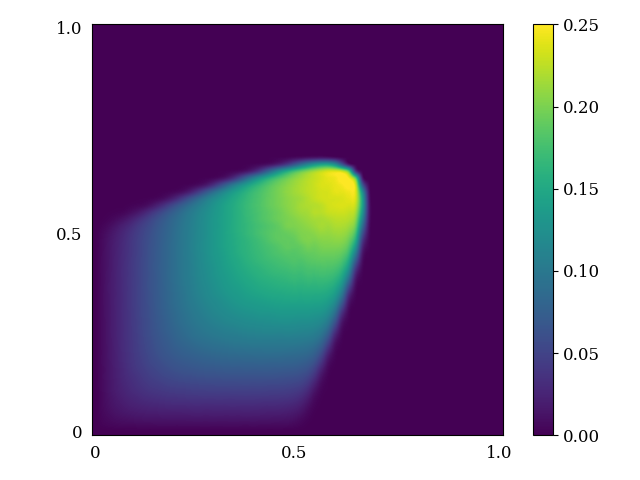
\includegraphics[trim = {0, 0, 3cm, 0}, clip, width=\textwidth]{X-rom-LE-SAE-15.png}
       \end{center}
            \caption{Solution $r = 15$}
        \end{subfigure}
   \begin{subfigure}[b]{0.23\textwidth}
       \begin{center}
        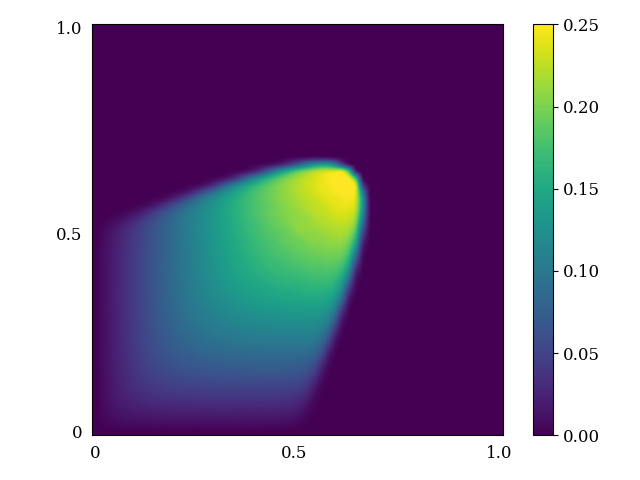
\includegraphics[trim = {0, 0, 3cm, 0}, clip, width=\textwidth]{X-rom-LE-SAE-20.png}
       \end{center}
            \caption{Solution $r = 20$}
        \end{subfigure}\\  
        \begin{subfigure}[b]{0.23\textwidth}
            \begin{center}
                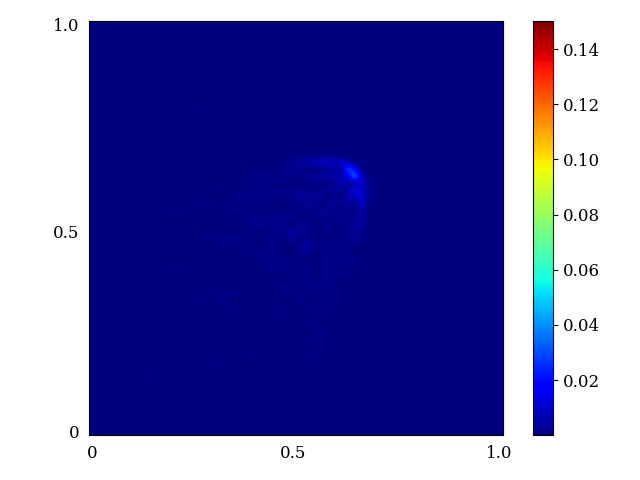
\includegraphics[trim = {0, 0, 3cm, 0}, clip, width=\textwidth]{X-rom-LE-SAE-5-abs-err.png}
            \end{center}
            \caption{Absolute error $r = 5$}
        \end{subfigure}  
        \begin{subfigure}[b]{0.23\textwidth}
            \begin{center}
                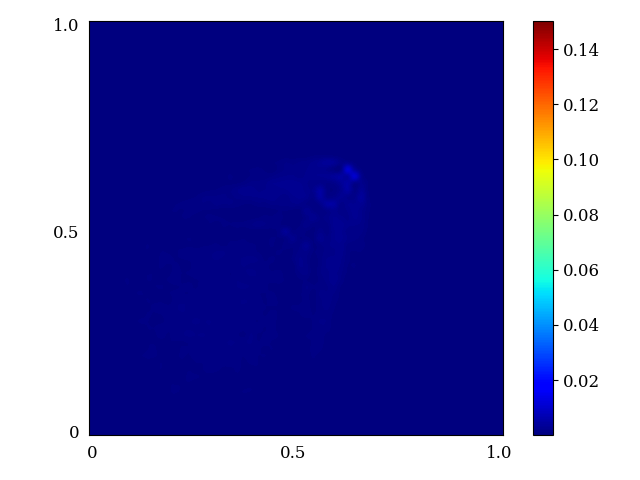
\includegraphics[trim = {0, 0, 3cm, 0}, clip, width=\textwidth]{X-rom-LE-SAE-10-abs-err.png}
            \end{center}
            \caption{Absolute error $r = 10$}
        \end{subfigure}   
        \begin{subfigure}[b]{0.23\textwidth}
            \begin{center}
                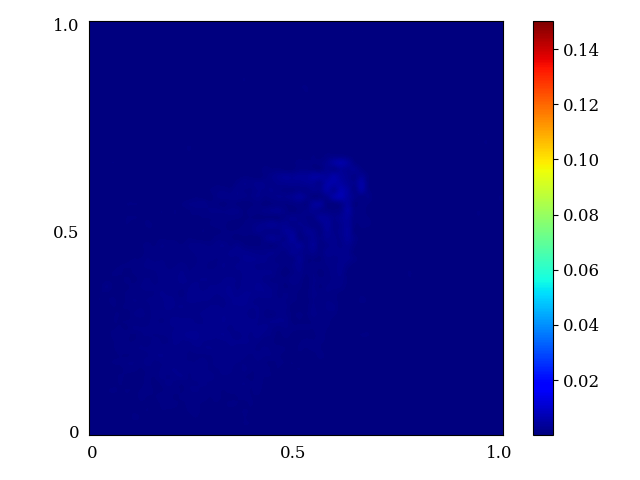
\includegraphics[trim = {0, 0, 3cm, 0}, clip, width=\textwidth]{X-rom-LE-SAE-15-abs-err.png}
            \end{center}
            \caption{Absolute error $r = 15$}
        \end{subfigure}    
        \begin{subfigure}[b]{0.23\textwidth}
            \begin{center}
                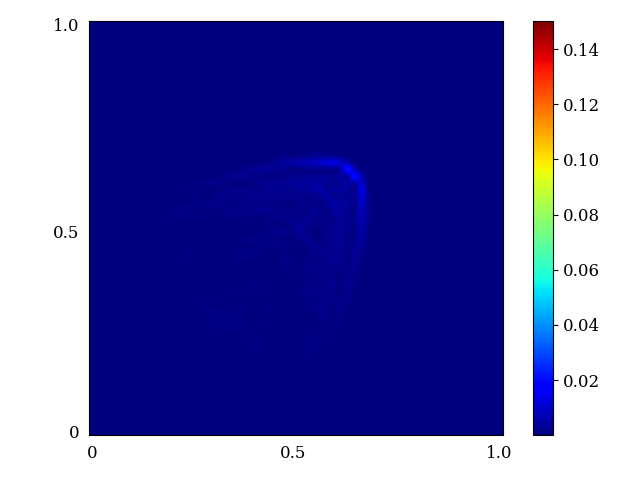
\includegraphics[trim = {0, 0, 3cm, 0}, clip, width=\textwidth]{X-rom-LE-SAE-20-abs-err.png}
            \end{center}
            \caption{Absolute error $r = 20$}
        \end{subfigure}
     \end{center}
     \caption[Solutions and pointwise errors for LE-SAE-DNNOp.]{Solutions (a, b, c, d) and pointwise errors (e, f, g, h) for LE-SAE-DNNOp with different latent space dimensions.}
        \label{fig: lesae-burger}
\end{figure}


\begin{figure}[!htb]
     \begin{center}
        \begin{subfigure}[b]{0.23\textwidth}
            \begin{center}
                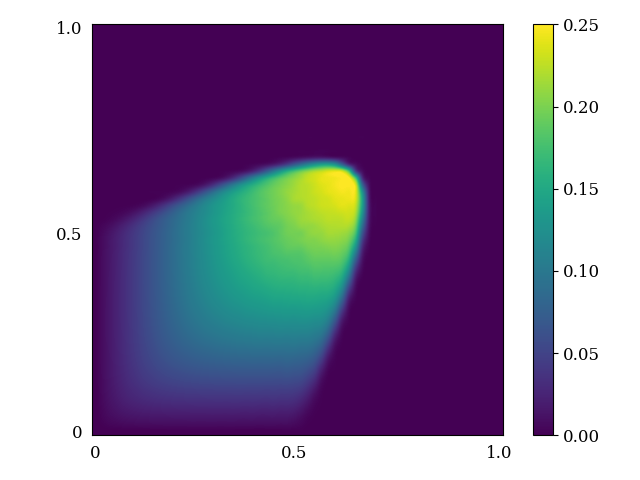
\includegraphics[trim = {0, 0, 3cm, 0}, clip, width=\textwidth]{X-rom-LE-CNNAE-5.png}
            \end{center}
             \caption{Solution $r = 5$}
         \end{subfigure}
    \begin{subfigure}[b]{0.23\textwidth}
            \begin{center}
                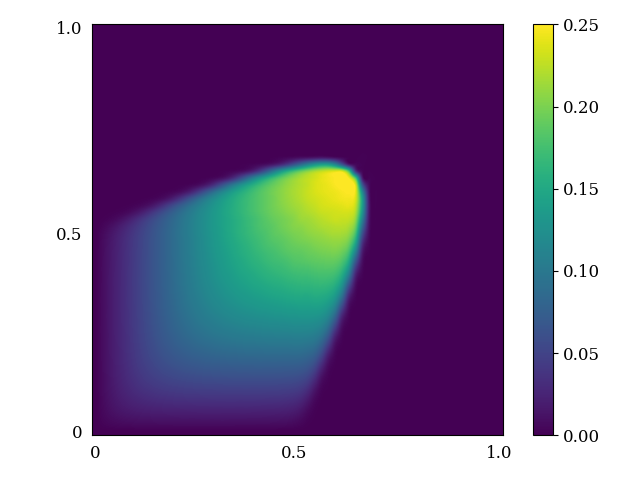
\includegraphics[trim = {0, 0, 3cm, 0}, clip, width=\textwidth]{X-rom-LE-CNNAE-10.png}
            \end{center}
             \caption{Solution $r = 10$}
         \end{subfigure}
    \begin{subfigure}[b]{0.23\textwidth}
            \begin{center}
                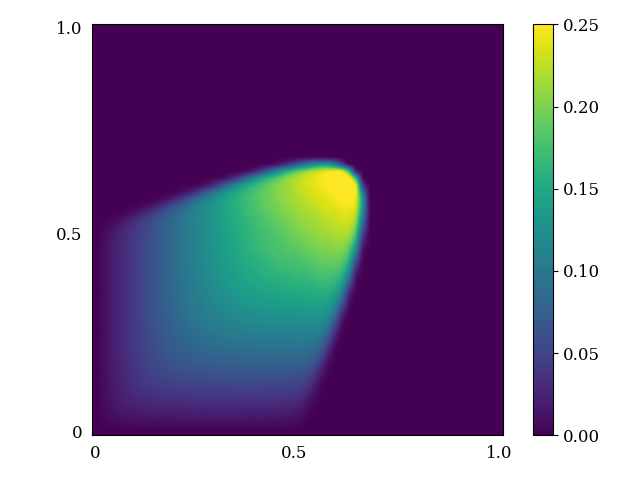
\includegraphics[trim = {0, 0, 3cm, 0}, clip, width=\textwidth]{X-rom-LE-CNNAE-15.png}
            \end{center}
             \caption{Solution $r = 15$}
         \end{subfigure}
    \begin{subfigure}[b]{0.23\textwidth}
            \begin{center}
                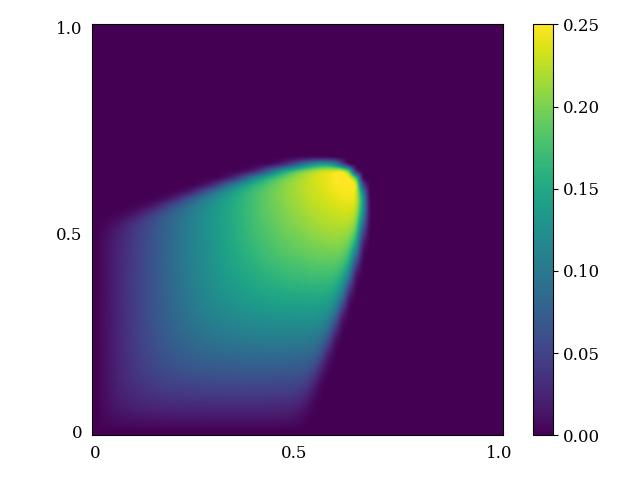
\includegraphics[trim = {0, 0, 3cm, 0}, clip, width=\textwidth]{X-rom-LE-CNNAE-20.png}
            \end{center}
             \caption{Solution $r = 20$}
         \end{subfigure}\\  
         \begin{subfigure}[b]{0.23\textwidth}
             \begin{center}
                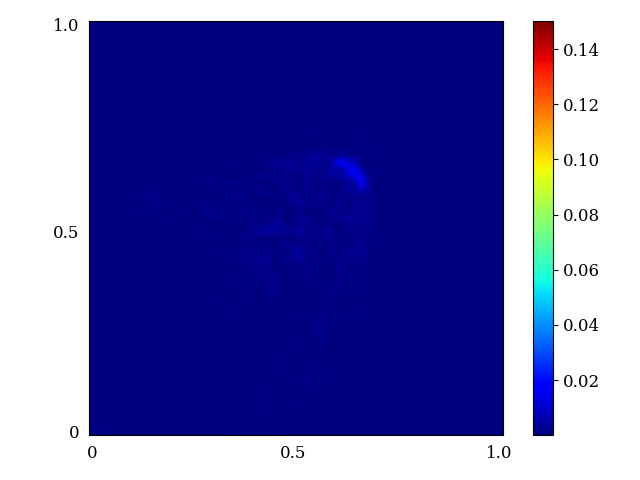
\includegraphics[trim = {0, 0, 3cm, 0}, clip, width=\textwidth]{X-rom-LE-CNNAE-5-abs-err.png}
             \end{center}
             \caption{Absolute error $r = 5$}
         \end{subfigure}  
         \begin{subfigure}[b]{0.23\textwidth}
             \begin{center}
                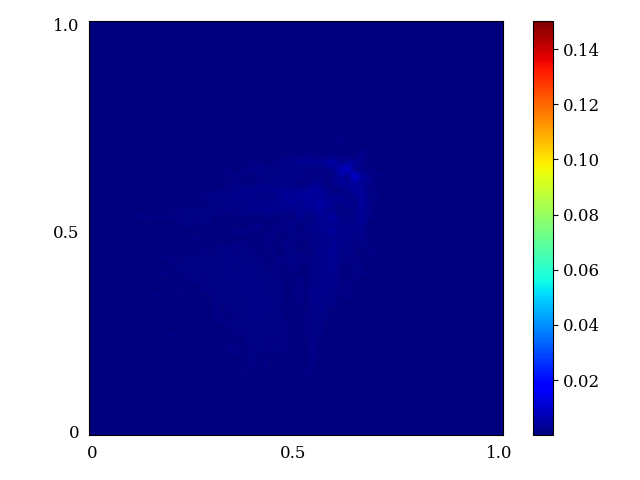
\includegraphics[trim = {0, 0, 3cm, 0}, clip, width=\textwidth]{X-rom-LE-CNNAE-10-abs-err.png}
             \end{center}
             \caption{Absolute error $r = 10$}
         \end{subfigure}   
         \begin{subfigure}[b]{0.23\textwidth}
             \begin{center}
                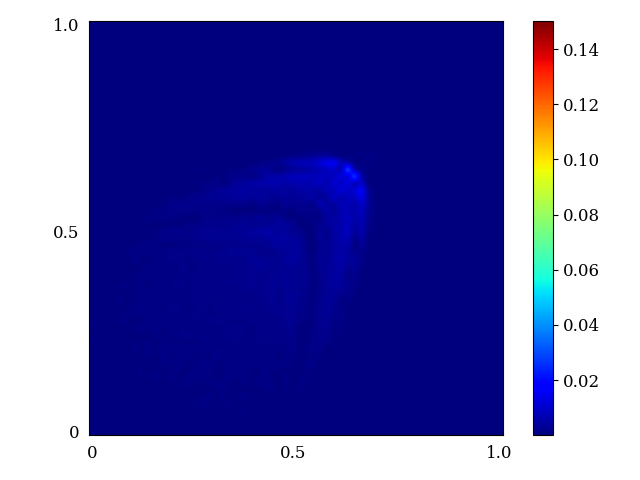
\includegraphics[trim = {0, 0, 3cm, 0}, clip, width=\textwidth]{X-rom-LE-CNNAE-15-abs-err.png}
             \end{center}
             \caption{Absolute error $r = 15$}
         \end{subfigure}    
         \begin{subfigure}[b]{0.23\textwidth}
             \begin{center}
                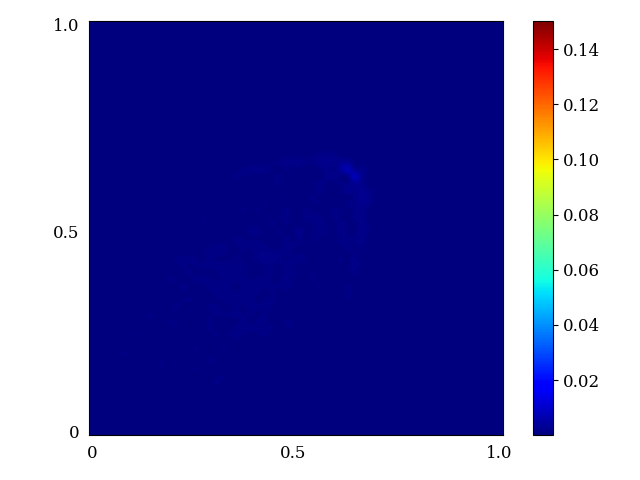
\includegraphics[trim = {0, 0, 3cm, 0}, clip, width=\textwidth]{X-rom-LE-CNNAE-20-abs-err.png}
             \end{center}
             \caption{Absolute error $r = 20$}
         \end{subfigure}
     \end{center}
     \caption[Solutions and pointwise errors for LE-CNNAE-DNNOp.]{Solutions (a, b, c, d) and pointwise errors (e, f, g, h) for LE-CNNAE-DNNOp with different latent space dimensions.}
        \label{fig: lecnnae-burger}
\end{figure}

\begin{figure}[!htb]
     \begin{center}
        \begin{subfigure}[b]{0.23\textwidth}
       \begin{center}
        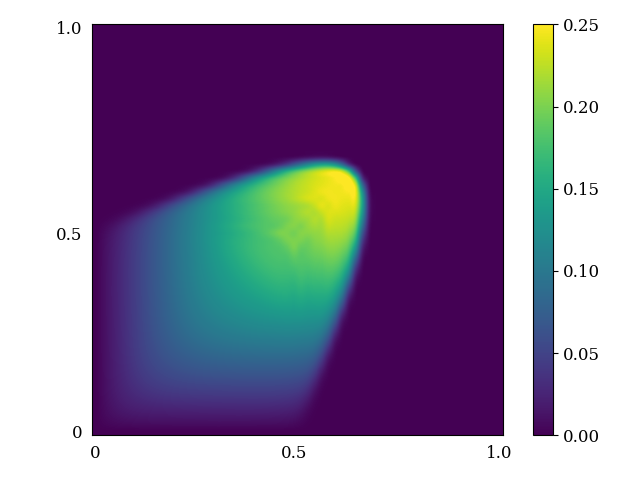
\includegraphics[trim = {0, 0, 3cm, 0}, clip, width=\textwidth]{X-rom-NE-DAE-5.png}
       \end{center}
            \caption{Solution $r = 5$}
        \end{subfigure}
   \begin{subfigure}[b]{0.23\textwidth}
        \begin{center}
            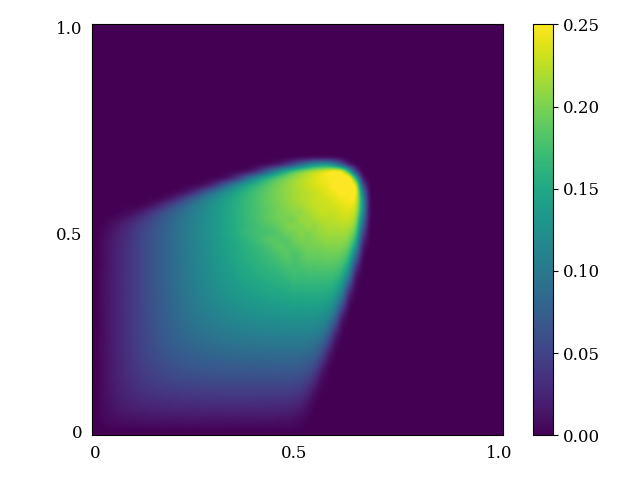
\includegraphics[trim = {0, 0, 3cm, 0}, clip, width=\textwidth]{X-rom-NE-DAE-10.png}
        \end{center}
            \caption{Solution $r = 10$}
        \end{subfigure}
   \begin{subfigure}[b]{0.23\textwidth}
            \begin{center}
                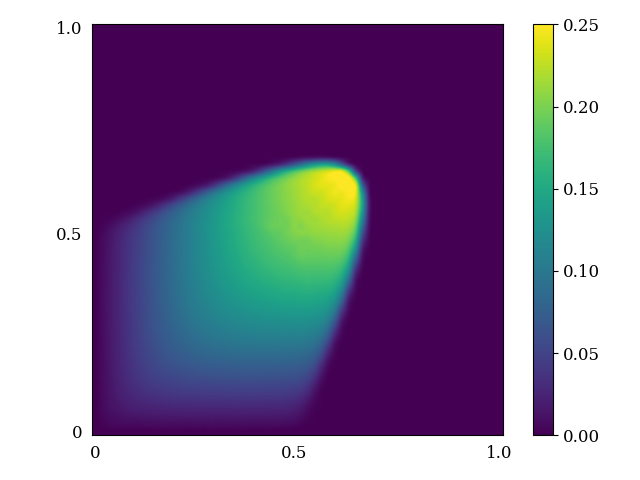
\includegraphics[trim = {0, 0, 3cm, 0}, clip, width=\textwidth]{X-rom-NE-DAE-15.png}
            \end{center}
            \caption{Solution $r = 15$}
        \end{subfigure}
   \begin{subfigure}[b]{0.23\textwidth}
            \begin{center}
                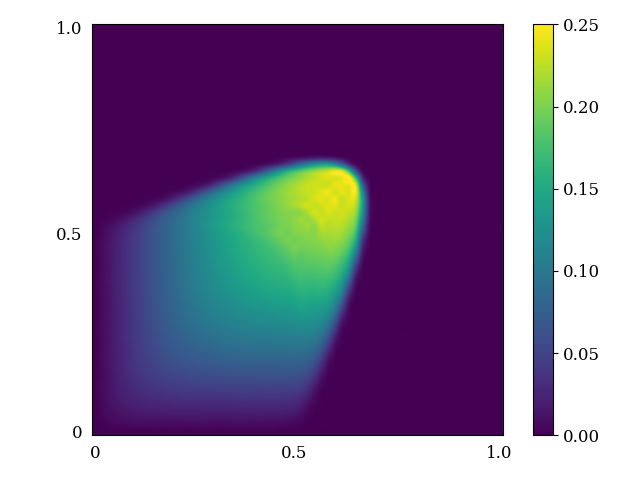
\includegraphics[trim = {0, 0, 3cm, 0}, clip, width=\textwidth]{X-rom-NE-DAE-20.png}
            \end{center}
            \caption{Solution $r = 20$}
        \end{subfigure}\\  
        \begin{subfigure}[b]{0.23\textwidth}
            \begin{center}
                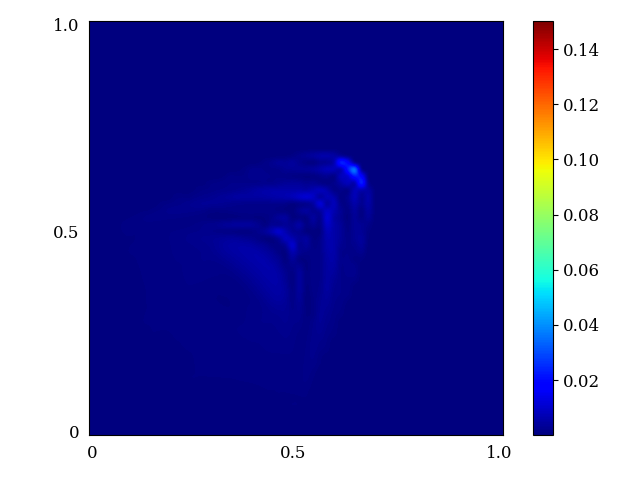
\includegraphics[trim = {0, 0, 3cm, 0}, clip, width=\textwidth]{X-rom-NE-DAE-5-abs-err.png}
            \end{center}
            \caption{Absolute error $r = 5$}
        \end{subfigure}  
        \begin{subfigure}[b]{0.23\textwidth}
            \begin{center}
                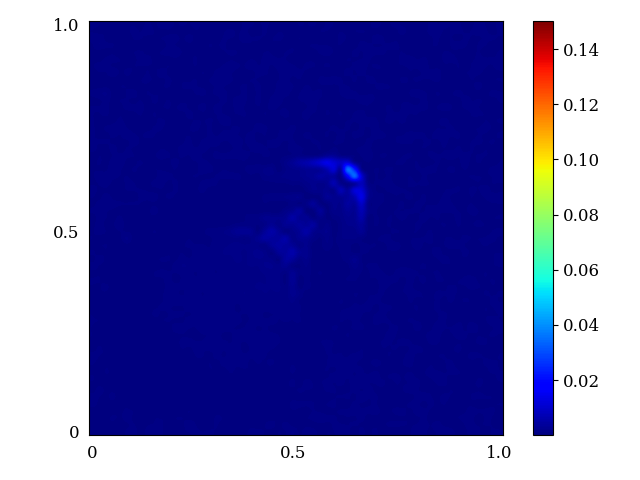
\includegraphics[trim = {0, 0, 3cm, 0}, clip, width=\textwidth]{X-rom-NE-DAE-10-abs-err.png}
            \end{center}
            \caption{Absolute error $r = 10$}
        \end{subfigure}   
        \begin{subfigure}[b]{0.23\textwidth}
            \begin{center}
            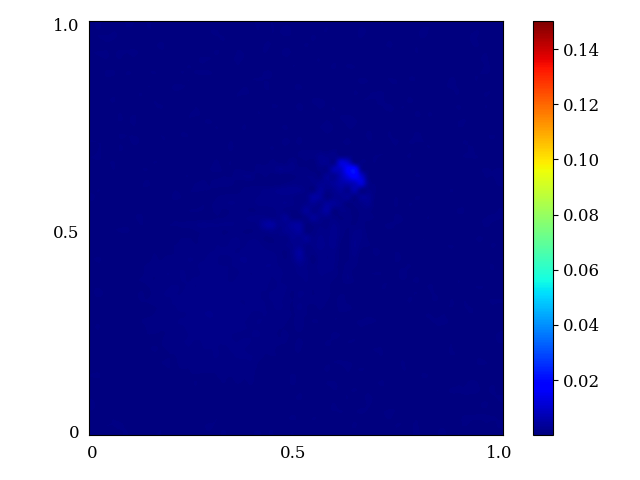
\includegraphics[trim = {0, 0, 3cm, 0}, clip, width=\textwidth]{X-rom-NE-DAE-15-abs-err.png}
            \end{center}
            \caption{Absolute error $r = 15$}
        \end{subfigure}    
        \begin{subfigure}[b]{0.23\textwidth}
            \begin{center}
                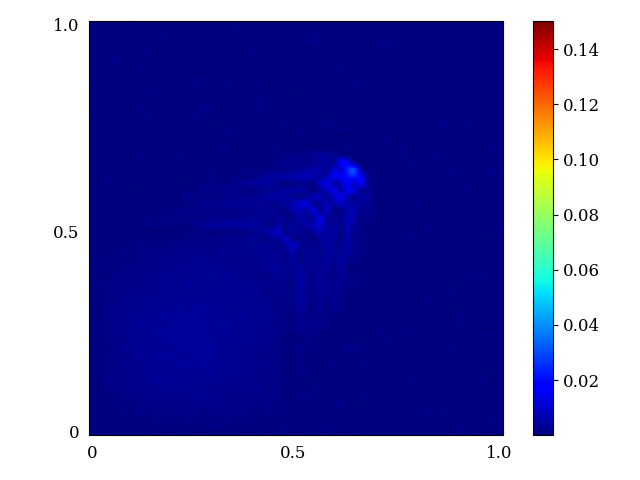
\includegraphics[trim = {0, 0, 3cm, 0}, clip, width=\textwidth]{X-rom-NE-DAE-20-abs-err.png}
            \end{center}
            \caption{Absolute error $r = 20$}
        \end{subfigure}
     \end{center}
     \caption[Solutions and pointwise errors for NE-DAE-DNNOp.]{Solutions (a, b, c, d) and pointwise errors (e, f, g, h) for NE-DAE-DNNOp with different latent space dimensions.}
        \label{fig: nedae-burger}
\end{figure}